\documentclass{cmc}
\usepackage{makecell}
\usepackage{enumitem}
\usepackage{amsmath}
\usepackage{float}
\usepackage{amsmath}
\usepackage{algorithm}
\usepackage[noend]{algpseudocode}
\makeatletter
\def\BState{\State\hskip-\ALG@thistlm}
\makeatother
\begin{document}

\pagestyle{fancy}
\lhead{\textit{\textbf{Computational Motor Control, Spring 2025} \\
    Final project, Project 1, GRADED}} \rhead{Student \\ Names}

\section*{Student names: \ldots (please update)}


\textit{
  \textbf{\corr{Deadline for Project 1: Sunday 27/04/2024 23:59}}
}

\section*{Motivations and project overview}\label{sec:exploring-swimming}

Zebrafish (\textit{Danio rerio}, Fig.~\ref{fig:zebrafish}) have emerged as a powerful model organism in biology and neuroscience, owing to their genetic tractability, transparent embryonic stages, and well-characterized spinal cord circuits. In adult zebrafish, locomotion can be generated across a range of swimming frequencies (slow, medium, and fast regimes), and the underlying neural control of these different speeds has become a central topic in vertebrate motor control research \cite{grillner2019current}.

\begin{figure}[H]
  \centering
  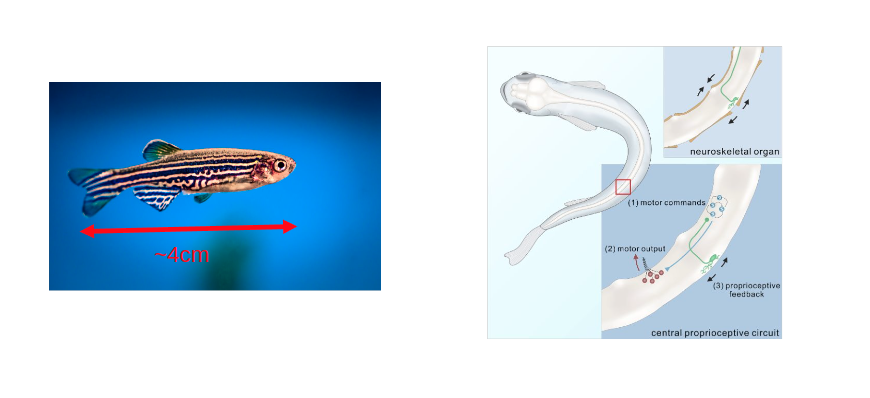
\includegraphics[width=1\textwidth]{figures/zebrafish.png}
  \caption[Zebrafish]{The zebrafish.}
  \label{fig:zebrafish}
\end{figure}

\noindent
\textbf{Scientific context and motivation.}
\begin{itemize}
\item \emph{Zebrafish as a model system.} Zebrafish offer a unique window into vertebrate locomotion. Their spinal cord circuitry is structurally simpler than that of larger vertebrates yet retains many fundamental features, including segmental organization and distributed central pattern generators (CPGs). This makes them ideal for studying the neural basis of rhythmic movements \cite{grillner2019current}.
\item \emph{Neuromechanical modeling.} A realistic neuromechanical model integrates neural control with the biomechanical properties of the fish body and its interaction with the fluid environment. Such a model allows us to systematically test how different neural parameters (e.g., activation frequencies, muscle stiffness, phase lags) affect locomotion performance \cite{ramdya2023neuromechanics}.
\item \emph{Proprioceptive feedback.} Recent findings highlight specialized stretch-sensitive organs in zebrafish musculature that can detect bending or strain along the body. How these sensors influence the fish’s ability to adapt swimming gaits—particularly when transitioning from slow to fast regimes or responding to environmental perturbations—remains an open question. Incorporating these sensors into a computational model can help clarify their role and importance \cite{picton_spinal_2021}.
\end{itemize}

\noindent
\textbf{Goals of this project.}

In \textbf{Project 1}, you will focus on modeling and simulating swimming in an adult zebrafish.
You will investigate how the muscle and body mechanics interact to produce efficient locomotion.
Additionally, you will design a CPG controller capable of generating the undulatory body movements required for propulsion.

In \textbf{Project 2}, you will extend this controller by incorporating \emph{proprioceptive feedback}, which has been experimentally shown to play a critical role in modulating swimming behavior based on local stretch signals along the body \cite{picton_spinal_2021}. Although proprioceptive feedback in zebrafish has been identified experimentally, its exact functional contribution to fine-tuning locomotion remains unclear. You will thus have the opportunity to integrate these newly discovered feedback loops into your simulation and test various hypotheses on how zebrafish sense and adapt to their environment.


The document is structured as follows:
\begin{enumerate}
  \item \textbf{Prerequisites.} A checklist of software dependencies and environment configurations needed before starting the project.
  \item \textbf{Code organization and usage.} Guidelines on how the provided Python files are structured and how to modify or extend them for your own experiments.
  \item \textbf{Mechanical model description.} A detailed explanation of the multi-segment zebrafish model, including the joints, muscle dynamics, and simplified fluid drag forces.
  \item \textbf{Exercises and questions.} A set of tasks guiding you through the study of different zebrafish controllers, muscle parameters and swimming kinematics.
\end{enumerate}

\noindent
By the end of these projects, you will have built a comprehensive simulation framework capable of generating biologically inspired swimming patterns in zebrafish. You will also have gained insight into the interplay between neural control, biomechanics, and sensory feedback in shaping locomotor behaviors, and you will be better equipped to address broader questions in motor control and bio-inspired robotics.

\noindent
\textbf{Instructions and deadlines.}

Update this \LaTeX \space file (or recreate a similar one, e.g.\ in Word) to prepare your answers to the questions. Feel free to add text, equations and figures as needed. Hand-written notes, e.g. for the development of equations, can also be included as pictures (from your cell phone or from a scanner). The code of project 1 should contain exercise 0 to 4.

The final report for this project should include:

\begin{itemize}
    \item A PDF file containing your responses to the questions.
    \item The source file of the report (*.doc/*.tex).
    \item The python code you used for the project.
\end{itemize}

All files should be inside a single zipped folder called \corr{final\_report\_name1\_name2\_name3.zip} where name\# are the team member's last names. \corr{Submit only one report per team}.



\section*{1. Prerequisites}
To have all the necessary python packages necessary to complete the
final project, check that you have installed all the necessary required packages.

\corr{\textit{IMPORTANT:}} Make sure you have activated and are using your
virtual environment and its python interpreter that that you have created for
this course.

\corr{\textit{NOTE:}} If you are unclear about the basic steps then refer back
to Lab 0 documentation

Next, pull the latest version of the exercise repository. Navigate to the
directory \textit{Project1/Python} in the terminal and execute the following,

\begin{lstlisting}[language=Bash]
  >> pip install -r requirements.txt --upgrade
\end{lstlisting}

We recommend that each group creates their own GitHub (or Gitlab) repository in order to easilty share code among the members. You can do that by copying the content of the \textit{Project1} folder into a newly created repository (e.g. $My\_CMC\_Project$).
\newline
\corr{Keep the repositories private and only share acces with other members of your team}.

Next, download the zip folder \textit{farms\_packages.zip} uploaded in Moodle and unzip its content in a dedicated directory (e.g. $My\_CMC\_Project/FARMS$). Open a terminal and navigate to that directory, then run the following commands:

\label{sec:mujoco-inst}
\begin{lstlisting}[language=Bash]
  >> pip install -e farms_core
  >> pip install -e farms_mujoco
  >> pip install -e farms_sim
  >> pip install -e farms_amphibious
\end{lstlisting}

This will install the \textit{MuJoCo} simulator and the \textit{dm\_control}
package which are software maintained by Deepmind for running multi-body rigid system
simulations. It will also install the \textit{farms\_core},
\textit{farms\_mujoco}, \textit{farms\_amphibious} and \textit{farms\_sim} FARMS packages developed at the
Biorobotics Laboratory (BioRob). If you are interested in knowing more about
\textit{MuJoCo} and FARMS, you can find out more on \href{https://mujoco.org/}{\corr{the
    official MuJoCo website}} and \href{https://www.biorxiv.org/content/10.1101/2023.09.25.559130v1https://www.biorxiv.org/content/10.1101/2023.09.25.559130v1}{\corr{the FARMS paper}}.


\subsection*{Example script}
You can now run a simulation example to get you accustomed
to the MuJoCo graphical interface with \corr{\textbf{example\_single.py}}.
Navigate to the Python directory of the project repository and try running:
\label{sec:first-example}
\begin{lstlisting}[language=Bash]
  >> python example_single.py
\end{lstlisting}

You should see the zebrafish model floating in the water. In the following sections, we will explain the properties of the mechanical model and how to design a controller to generate swimming locomotion.

\subsection*{Graphical User Interface Interaction}
When you run the example script, a Graphical User Interface (GUI) should launch.
You can use the left mouse click to move around the scene and right mouse click
to rotate the camera. You can also select a part of the model by double left
clicking on a part. Once selected, you can then interact with it by holding the
CONTROL key and dragging with left or right click. Try it out for yourself to
familiarise with the interface.

There are many keyboard shortcuts also available

\begin{itemize}
\item Press SPACE to toggle play/pause
\item Press ``\textquotesingle'' / ``\textsuperscript{$\wedge$}'' to change
  speed factor (between zero (0) and backspace)
\item Press w to toggle wireframe
\item Press t to toggle transparency
\item Press s to toggle shadows
\item Press c to show collisions
\item Press f to show collisions forces, combine with p to show
  friction/reaction
\item Press b to show external forces (try in water later on)
\item And many more...
\end{itemize}

\section*{2. Code organization and usage.}\label{subsec:code}

In this project you will modify the files \fileref{exercise\_\#.py}, \fileref{controllers/wave\_controller.py}, \\
\fileref{controllers/abstract\_oscillator\_controller.py}, \fileref{simulation\_parameters.py} (optional) \\ and \fileref{plot\_results.py} (optional). We provide below
a brief description of these and the other files, for completeness.

\begin{itemize}
\item \corr{\textbf{example\_single.py}} --- Run single simulation example (fixed parameters)
\item \corr{\textbf{example\_multiple.py}} --- Run multiple parallel simulations with different parameters
\item \corr{\textbf{exercise\_\#.py}} --- Files for the exercises 1-3
\item \corr{\textbf{controllers/wave\_controller.py}} --- This file contains the equations for the left and right muscle activations in a step function, which is internall called at each iteration time step.
\item \corr{\textbf{controllers/abstract\_oscillator\_controller.py}} --- Contains the equations for the abstract oscillator neural controller. You have to implement here the differential equations that will be described later in the code.
\item \corr{\textbf{simulation\_parameters.py}} --- This file contains the
  SimulationParameters class and is provided for convenience to send parameters
  to the setup of the controller. Please carefully read the parameter list
  and their documentation in this code.
\item \corr{\textbf{metrics.py}} --- This file contains the implementation
  for all the controller/mechanical metrics (see below).
\item \corr{\textbf{plotting\_common.py}} --- Plotting utilities (see below).
\item \corr{\textbf{plot\_results.py}} --- Loading and plotting the simulation results.
\item \corr{\textbf{logs folder}} --- Contains all the simulation logs
\item \corr{\textbf{util folder}} --- Contains all the utilities for running the simulation (\textbf{do not modify})
\item \corr{\textbf{muscle\_parameters folder}} --- Contains the optimized muscle parameters used in the Project (\textbf{do not modify})
\item \corr{\textbf{models folder}} --- Contains extra code for the biomechanical and simulation in MuJoCo (\textbf{do not modify})
\end{itemize}


\subsection*{Running the simulations}\label{subsec:simulating}
We provided two example files for running the simulations:
\begin{itemize}
\item \fileref{example\_single.py} - in this example you can see how to run a single simulation of the zebrafish. You can explore the GUI, where to store the simulation data (for postprocessing and plotting) and how to use some plotting tools (explained more in the next section).
Try to change some parameters of the \fileref{SimulationParameters.py:SimulationParameters()} class to test how it works (try, i.e. to save the video, activate/deactivate the headless mode, etc). The results are saved to \textbf{controller} variable and \textbf{log\_path} folder for further inspection and analysis. The results store the sensor readings (check \fileref{utils/run\_closed\_loop:run\_single()}) and the controller states (Class variables in your controller, i.e. \fileref{controllers/wave\_controller.py}, \fileref{controllers/abstract\_oscillator\_controller.py}).



\item \fileref{example\_multiple.py} - in this example you can see how to run multiple simulation (without GUI) in parallel using the processors for different parameter values.
\end{itemize}


\subsection*{Plotting tools}\label{subsec:plotting}
We provided some optional plotting tools in \fileref{plotting\_common.py} (check the documentation for more details):
\begin{itemize}
\item \fileref{plot\_time\_histories} - plots time histories of a vector of states on a single plot
\item \fileref{plot\_time\_histories\_multiple\_windows} - plots time histories of a vector of states on multiple subplots
\item \fileref{plot\_left\_right} - plotting left and right time histories on separate subplots
\item \fileref{plot\_2d} - plots an array 2d colored plot (uuseful for 2d parameter searches)
\item \fileref{plot\_trajectory} - plots head positions
\item \fileref{plot\_positions} - plots positions of the links

Examples for how to use these tools can be found in \fileref{example\_single.py} and \fileref{plot\_results.py}

\end{itemize}



\subsection*{Performance metrics}\label{sec:performance-metrics}

In \corr{\textbf{util.metrics.py}}, we provide some basic functions to evaluate the performance
of the model simulations, and stored in the dictionary \corr{wave\_controller.py::WaveController.metrics}.

In order to quantitatively evaluate both the neural controller and the mechanical body of the zebrafish model, we define a series of metrics that capture different aspects of locomotor performance. These metrics are computed over the last portion of the simulation (e.g.\ the final 60\% of the recorded data) to avoid transient effects. Below, we provide a brief description of each metric category—\emph{neural} and \emph{mechanical}—and present the main equations used in the code.

\subsubsection*{Neural metrics}

The \textbf{neural metrics} focus on signals generated by the controller (e.g., muscle activations). Typically, we analyze the difference $x_i = M^i_{L} - M^i_{R}$ between left- and right-side muscle commands, which directly relates to the torque output around each joint $i$.

\begin{itemize}
  \item \textit{Neural frequency} (\(f_{\mathrm{neur}}\)).
  We compute the neural frequency via a Fast Fourier Transform (FFT) of the muscle activation signals.
  \[
    f_{\mathrm{neur}} = < \underset{f}{\mathrm{argmax}}\;\bigl|X_i[f]\bigr| >_i
  \]


  \item \textit{Neural amplitude} (\(A_{\mathrm{neur}}\)).
  The amplitude is estimated as:
  \[
    A_{\mathrm{neur}} = <\frac{2\,\bigl|X_i[k^i_{\text{max}}]\bigr|}{N} >_i
  \]
  where \(\bigl|X_i[k^i_{\text{max}}]\bigr|\) is the magnitude of the FFT at the index corresponding to the dominant frequency for each signal, and \(N\) is the number of samples.


  \item \textit{Intersegmental phase lag ($IPL_{neur}$).}
  For two oscillatory signals \(x_1(t)\) and \(x_2(t)\) with similar frequencies,
  the delay \(\Delta t_{1,2}\) is computed by cross-correlation:
  \[
    \Delta t_{1,2}\;=\;\underset{\tau}{\mathrm{argmax}}\;\bigl(\mathrm{corr}\bigl(x_1,\,x_2\bigr)\bigr)
  \]

  The corresponding phase lag is computed by normalizing the delay by the average frequency of the two signals \(f_{1,2}\), as:
  \[
    PL_{1,2} \;=\; 2\pi\,f_{1,2}\;\Delta t,
  \]

  Finally, the overall intersegmental phase lag is computed by averaging the phase lag values for each successive couple of signals along the body:

    \[
    IPL_{neur} \;=\; \frac{1}{N-1} \sum_{i=0}^{n-2} PL_{i, i+1}
  \]

  \item \textit{Total wave lag} ($TWL_{neur}$).
  The total wave lag is obtained by summing these pairwise lags along the body and normalizing by the fraction of the body that is actively driven by joints:
  \[
    TWL_{neur} \;=\;\frac{(N-1) IPL}{\text{active\_body\_fraction}}.
  \]


\end{itemize}

\subsubsection*{Mechanical metrics}.

The \textbf{mechanical metrics} quantify how effectively and efficiently the body segments move in the simulated fluid environment. They rely on joint angles, joint torques, link positions, and center-of-mass trajectories.

\begin{itemize}
  \item \textit{Mechanical frequency ($f_{mech}$) and amplitude ($A_{mech}$).}
  These metrics are computed analogously to their neural counterparts, considering the joint angles instead of the muscle commands. In the metrics dictionary we give you access to both the vector containing all 15 joint frequencies and amplitudes ($metrics["mech\_joint\_frequencies"]$/$metrics["mech\_joint\_amplitudes"]$) and the average across all joints ($metrics["mech\_mean\_frequency"]$/$metrics["mech\_mean\_amplitude"]$).


  \item \textit{Forward speed ($v_{fwd}$) and lateral speed ($v_{lat}$).}
  At each time step, we project the center-of-mass velocity \(\mathbf{v}_{\mathrm{COM}}(t)\) onto the forward ($d_{fwd}(t)$) and lateral ($d_{lat}(t)$) principal axes of the fish.
  The overall speed metrics are computed by averaging the instantaneous values over time:

  \[
    v_{\mathrm{fwd}} \;=\; <\mathbf{v}_{\mathrm{COM}}(t)\,\cdot\,\mathbf{d} _{\mathrm{fwd}(t)} >_t
  \]
  \[
    v_{\mathrm{lat}} \;=\; <\mathbf{v}_{\mathrm{COM}}(t)\,\cdot\,\mathbf{d}_{\mathrm{lat}(t)} >_t
  \]

  \item \textit{Sum of torques} (\(T_{\mathrm{sum}}\)).
  We sum the absolute value of the net torques on all active joints:
  \[
    T_{\mathrm{sum}} \;=\; dt \times \sum_{t}\sum_{j=1}^{n_\mathrm{joints}} \bigl|\tau_j(t) \bigr|.
  \]

  \item \textit{Energy consumption (\(E\)).}
  The code integrates the positive power \(\tau_j(t)\,\dot{\theta}_j(t)\) at each joint:
  \[
    P_j(t) \;=\;\max\bigl( \; \tau_j(t)\,\dot{\theta}_j(t),\, \;0 \bigr)
  \]
  \[
    E \;=\;  dt \times \sum_{t} \sum_{j=1}^{n} P_j(t)
  \]
  By taking only positive contributions, we model that active muscles do not \emph{recover} energy from negative work.

  \item \textit{Cost of transport (CoT).}
  The cost of transport relates the energy expenditure to the distance traveled. In our simplified code, it is:
  \[
    \text{CoT} \;=\;\frac{E}{D_{\mathrm{fwd}}},
  \]
  where \(D_{\mathrm{fwd}}\) is the forward distance covered by the center of mass.

  \item \textit{Trajectory curvature (\(\kappa\)).}
  To measure how much the fish’s center of mass bends its path in the \(xy\)-plane, we compute
  \[
    \kappa \;=\;\frac{x''(t)\,y'(t)\;-\;x'(t)\,y''(t)}{\bigl(x'(t)^2 + y'(t)^2\bigr)^{3/2}},
  \]
  where \(\bigl(x(t),\,y(t)\bigr)\) is the COM trajectory. The code averages \(\kappa\) over each swimming cycle to produce \(\text{mech\_traj\_curv}\).

  \item \textit{Mechanical phase lag ($IPL_{mech}$) and total wave lag ($TWL_{mech}$).}
  These metrics are computed analogously to their neural counterparts, considering the joint angles instead of the muscle commands.

\end{itemize}

\noindent
\textbf{Putting it all together.} The code collects both sets of metrics into a single dictionary via the \texttt{compute\_all\_metrics} function. By analyzing these metrics, one can characterize how effectively the controller drives the fish (neural side) and how well the fish converts these signals into forward locomotion (mechanical side). This framework thus provides a quantitative basis for comparing different parameter choices, controller designs, and muscle models throughout the project. The code also provides additional functions that you may use as a basis for defining any other metrics that you consider useful for the analyses.

\subsection*{Pro tips}\label{subsec:tips}

\begin{itemize}
\item \corr{\textbf{Check the notes on the code}}. Many explanations are given therein.
\item \corr{Be concise and precise in the answers} in the answers of the exercises.
\item You can \corr{append videos to explain your reasoning}.
\end{itemize}

% \newpage

%%%%%%%%%%%%%%%%%%%%%%%%%%%%%%%%%%%%%%%%%%%%%%%%%%%%%%%%%%%%%%%%%%%%%%%%%%
% MECHANICAL MODEL %%%%%%%%%%%%%%%%%%%%%%%%%%%%%%%%%%%%%%%%%%%%%%%%%%%%%%%
%%%%%%%%%%%%%%%%%%%%%%%%%%%%%%%%%%%%%%%%%%%%%%%%%%%%%%%%%%%%%%%%%%%%%%%%%%

\section*{3. Mechanical model description}\label{sec:mechanical}
The mechanical zebrafish model consists of $n_{links}=16$ links connected by $n_{joints}=15$
rotational yaw joints (see Fig\ref{fig:mechanical}). The joints are numbered from 0 to 14, ordered from the head to the tail.

The torque produced by each joint is computed by means of Ekeberg Muscle Models (\ref{fig:mechanical}).
For each joint $i=0,...,14$, the model receives in input the left ($M_{L_i}$) and right ($M_{R_i}$) activations from the muscle cells, the current joint angle ($\theta_i$) and joint speed ($\Dot{\theta_i}$) to compute the resulting output torque ($\tau_i$) via:

  \[
	\tau_i = \alpha_i M_{diff_i} + \beta_i(\gamma_i +M_{sum_i} )\theta_i + \delta_i \Dot{\theta_i} \\
  \]
  \[
    M_{diff_i} = (M_{L_i} - M_{R_i}) \\
  \]
  \[
    M_{sum_i} = (M_{L_i} + M_{R_i})
  \]

Where $\alpha_i$ is the active gain, $\gamma_i$ is the passive stiffness, $\beta_i$ is the active stiffness, $\delta_i$ is the damping coefficient. The Ekeberg muscle model is a rotational spring-damper system with the addition of a variable stiffness term $\beta (M_L+M_R) \theta_i$. The active term of the model acts an external torque $\alpha(M_L-M_R)$.

The Ekeberg model parameters have been optimized in order to obtain a target resonance frequency and damping ratio for small angular deflections. Details about the optimization procedure can be found in the supplementary material of \cite{pazzaglia2025balancing}.
The muscle\_parameters folder contains the results of the optimization for several combinations of the target parameters. You will study different combinations in order to understand their effect on the swimming performance.

When submerged in water, the body is subjected to buoyancy and hydrodynamic forces. Buoyancy forces are applied to each link according to its submerged volume $V_{UW}$

  \[
	\mathrm{F_{b_i}} = V_{UW_i} \rho g
  \]

Where $\rho$ is the water density and $g$ is the gravity acceleration ($g = 9.81 m/s^2$).
Since adult zebrafish typically swim in high Reynolds number regimes, we opted for a simplified hydrodynamic model composed of inertial drag forces. For each link, a speed dependent drag force ($F_d$) is applied in each dimension ($i$) according to:

  \[
	\mathrm{F_{d_i}} = \frac{1}{2} \rho C_{d_i} A_{i} V_{i}^2
  \]

Where $A$ is the link's cross-sectional area, $c_{d_i}$ is the drag coefficient in the i-th dimension, $V_{i}$ is the current speed of the link in the i-th dimension in the reference frame of the center of mass of the link. The drag coefficients were chosen in order to match the mechanical metrics computed from swimming zebrafishes.



\begin{figure}[ht]
  \centering 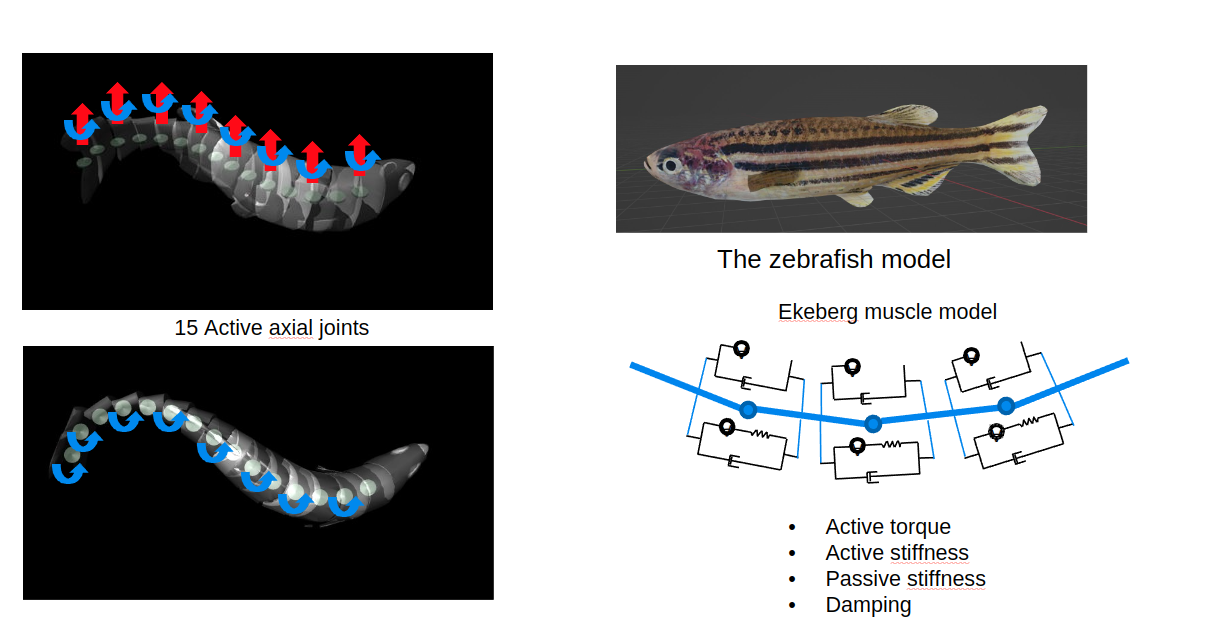
\includegraphics[width=1.0\textwidth]{figures/mechanical.png}
  \caption{\label{fig:mechanical} The mechanical model of the zebrafish}
\end{figure}

\newpage





%%%%%%%%%%%%%%%%%%%%%%%%%%%%%%%%%%%%%%%%%%%%%%%%%%%%%%%%%%%%%%%%%%%%%%%%%%
% QUESTIONS %%%%%%%%%%%%%%%%%%%%%%%%%%%%%%%%%%%%%%%%%%%%%%%%%%%%%%%%%%%%%%
%%%%%%%%%%%%%%%%%%%%%%%%%%%%%%%%%%%%%%%%%%%%%%%%%%%%%%%%%%%%%%%%%%%%%%%%%%

\newpage
\section*{4. Exercises and questions}
At this point you can now start to work on implementing your exercises 1-4 below (use \textbf{exercise1.py}-\textbf{exercise4.py} to solve the exercises).

\subsection*{1. Wave Controller} \label{subsec:wavecontroller}
Implement a sine wave swimming controller that generates a periodic traveling wave for activations of the left and right muscles ($M_{L_i}$ and $M_{R_i}$, for $i=0,...14$) to activate the zebrafish according to equation \ref{eq:sine_controller}. Write your implementation in \fileref{exercise\_0.py}. Plot the time evolution of the joint angles, center of mass trajectory in 2d (x,y) space, and motor outputs of the left and right oscillators.

\begin{eqnarray}
  \label{eq:sine_controller}
M_{L_i} (t)&=0.5 + \frac{A}{2} \cdot \sin \left( 2 \pi \left( f \cdot t - TWL \cdot \frac{i}{N_{joints}} \right) \right)  \nonumber \\
M_{R_i} (t)&=0.5 - \frac{A}{2} \cdot \sin \left( 2 \pi \left( f \cdot t - TWL \cdot \frac{i}{N_{joints}} \right) \right)
\end{eqnarray}
where $TWL$ is the total wave lag, $A$ is the amplitude and $f$ is the frequency of the wave. Note that that equation \ref{eq:sine_controller} guarantee that the active stiffness component $M_{sum_i} = (M_{L_i} + M_{R_i})$ is equal to 1 at all times, and that the muscle activation difference $M_{diff_i} = (M_{L_i} - M_{R_i})$ has amplitude $A$.



\textbf{\underline{Question 1} Test the controller's ability to generate swimming locomotion for fixed values of $\epsilon \in [0,2]$, $A \in [0,2]$ and $f \in [1,5] Hz$ (test different parameter combinations). Show plots of the left and right muscle activations $M_{L_i}$ and $M_{R_i}$, and of the animal head trajectory in the (x,y) plane. Also, show the evolution of the joint angles. Report the performance metrics in your report. }


\subsection*{2. Muscle Optimization}
The mechanical behavior of muscle tissue can be approximated by simple passive elements such as springs and dampers (read paper \cite{tytell2014role} up to page 51). These elements, when combined properly, allow us to study the behavior of muscle under compressive and tensile loads. In this section you will explore the ability to test if and how passive properties of the muscles can be used to improve the performance of the zebrafish swimming behavior in combination with the muscle actuation.

\subsubsection*{A simple spring mass damper pendulum example}

\begin{figure}[H]
  \centering 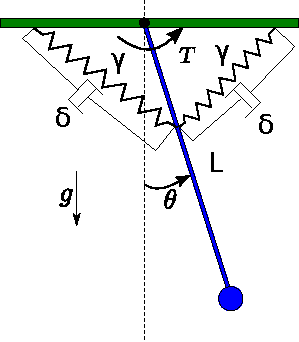
\includegraphics[width=0.2\textwidth]{figures/pendulum.pdf}
  \caption{\label{fig:pendulum} A pendulum with passive elements.}
\end{figure}
Let us consider a standard spring-damper pendulum (Fig \ref{fig:pendulum}), whose angle from the vertical $\theta$ follows the follows dynamics:

\begin{equation}
    I \ddot{\theta} = -\gamma \theta - \delta \dot{\theta} - mgL\sin(\theta),
    \label{pendulum}
\end{equation}
where $L$ is the length of the pendulum, $m$ the mass, $g$ the gravity, $\gamma$ the stiffness of the spring, and $\delta$ the damping coefficient. Lastly, let us consider the inertia $I=mL^2$.

\textbf{\underline{Question 2.1} Derive the approximation of \ref{pendulum} for small angles such as:
$$ \ddot{\theta} + 2 \xi \omega_r \dot{\theta} + \omega_r^2 \theta = 0. $$
Where here $\xi$ is called the damping ratio and $\omega_r$ the (undamped) natural frequency of the spring mass damper. Find a combination of parameters $m$, $L$, $\gamma$ and $\delta$ that gives underdamped, critically damped and underdamped conditions.}


This approach allows us to prescribe to a single muscle a desired resonant frequency and damping ratio. Similar to a single muscle, we can model a chain of muscles, as in the case of the zebrafish model proposed in this project, to have a desired resonant frequency and damping ratio using a system identification approach \cite{pazzaglia2025balancing}. In this project you will not implement this method but we give you access to a set of muscle parameters values of each joint $\alpha_i$, $\gamma_i$, $\beta_i$ and $\delta_i$ that are tuned to have the same target resonant frequency $\omega_r$ and damping ratio $\xi$ (the details of the method can be found in the Supporting information file S3 in \href{https://journals.plos.org/ploscompbiol/article?id=10.1371/journal.pcbi.1012101}{this link}).


The muscle parameters of each joint are tuned to have the same target resonant frequency $\omega_r$ and damping ratio $\xi$. The parameters used in the simulation are stored in files in the folder \textbf{muscle\_parameters}. Each of these files can be selected for simulation by selecting the the $muscle\_parameters\_tag$ argument in \textit{simulation\_parameters.py} file. For example, the file
$$ muscle\_parameters\_FN\_6000\_ZC_1000\_G0\_419 $$
contains the muscle parameters with resonant frequency $\omega_r=6$Hz and damping ratio $\xi=1$ and can be selected in \textit{simulation\_parameters.py} by adding the entry
$$ muscle\_parameters\_tag = 'FN\_6000\_ZC\_1000\_G0\_419' $$
This is the default parameter setting for the simulation.

We also provide a multiplication factor called \textit{damping\_factor} in the simulation parameter that scales the damping ratio by $damping\_factor*damping\_ratio$ and allow you to test different muscle properties (underdamped, critically damped and overdamped muscles).

In this exercise you will use the following simulation settings:
\begin{enumerate}
    \item Set no gravity mode, by setting the vectory gravity parameter = $gravity = np.array([0,0,0])$.
    \item Set a predefined initial joint configuration $joint\_poses = 0.3*np.ones(15)$. With this configuration all the joint angles are initially at $0.3 \pi$ by setting
    \item In this exercise you will test two different animal positions, by using two different values of $animal\_pose = [0.0, 0.0, -0.01, 0.0, 0, -1.570796327]$ (the default value) and $animal\_pose = [0.0, 0.0, -0.01, 0.0, 0, -1.570796327]$. In the first pose the animal is positioned in water, and therefore is affected by the drag water forces. In the second set of positions the animal is located 10 meters above ground (in ``space``), and it is therefore not affected by water forces.
    \item Write your implementation in \fileref{exercise\_1.py}
\end{enumerate}

\textbf{\underline{Question 2.2}. Run a simulation of the fish 10 meters above ground with no gravity and test different values of DR $\in {1,0.3,0.1}$ with no controller (amp=0). What do you observe? Are your findings in line with the analysis of question 2.1? }



\textbf{\underline{Question 2.3}. Run a systematic simulation study of the effect of adding the wave controller you implemented in Question 1 as a forcing term for the muscle model. Run multiple simulations of the controller with fixed amplitude amp=0.01 and vary the controller frequency $\in \left( 0,20 \right)$ for TWL=0 (0 total wave lag). Compute and plot the mean amplitudes across all the joints (stored in metrics["mech\_joint\_amplitudes"] as a function of the controller frequency for different damping ratios DR $\in \{1,0.3,0.1\}$. Repeat the analysis in water and in space (w/o drag forces). Repeat the same analysis also for TWL=0.5. What conclusions can you derive, in relation to the paper \cite{tytell2014role}? How could the system benefit from the passive properties to swim more efficiently?
}




\subsubsection*{Relationship between muscle properties and swimming performance}

In \cite{ampatzis2014separate}, the authors demonstrated that the zebrafish locomotor networks can be subdivided into three modules, each one specialized for a different frequency range. Interestingly, this compartmentalization involves the neurons of the CPG network, as well as the motoneurons and the corresponding muscle cells \cite{grillner2019current} (see Fig\ref{fig:speed_modules}).

\begin{figure}[H]
  \centering 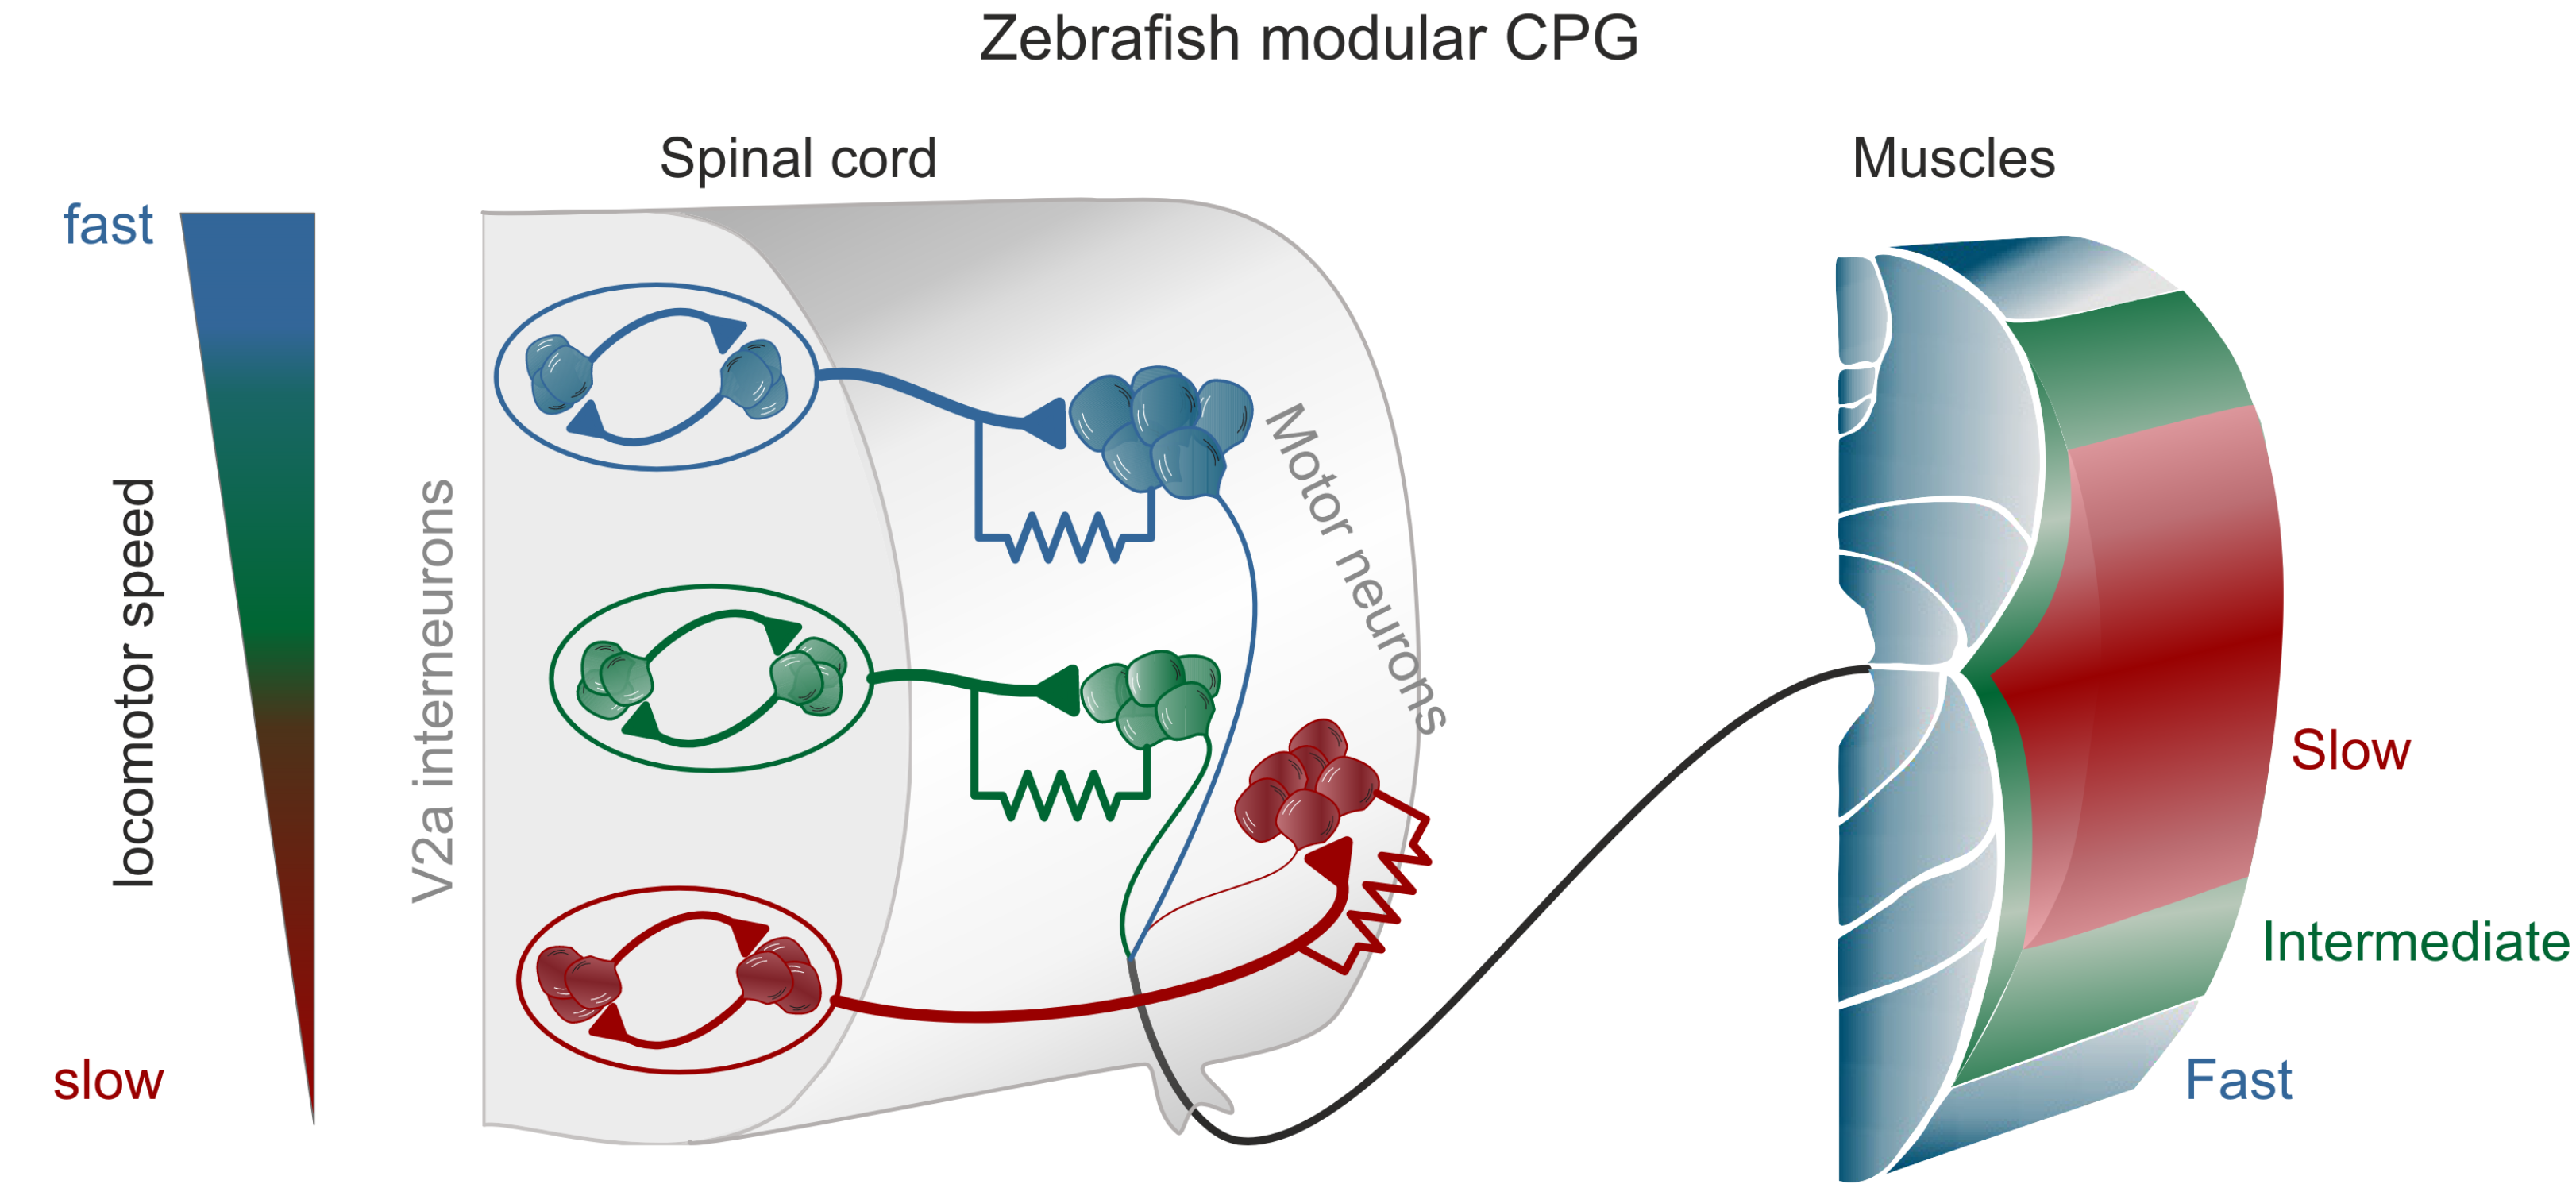
\includegraphics[width=0.5\textwidth]{figures/zebrafish_modular_network.png}
  \caption{\label{fig:speed_modules} A schematic of the modular organization of the locomotor circuits in the adult zebrafish.}
\end{figure}

In this section, you will study the relationship between the selected muscle parameters and the resulting swimming performance.
You will study at least three different muscle parameters configurations, namely:
\begin{itemize}
    \item FN\_5000\_ZC\_1000\_G0\_419
    \item FN\_7500\_ZC\_1000\_G0\_419
    \item FN\_10000\_ZC\_1000\_G0\_419
\end{itemize}

\textbf{\underline{Question 2.4}}.For each muscle parameters configuration, study the relationship between the activation frequency and the total wave lag (TWL) of the control wave. Change the activation frequency in the range $[3.0, 40.0] Hz$, corresponding to the range observed experimentally in fishes. Change also the total wave lag in the range $[0.0, 2.0]$. Set the amplitude of the controller to a constant value of $0.5$ for all joints. Report the results obtained repeating the analysis for the three muscle combinations:

\begin{itemize}
    \item \textbf{What is the optimal TWL to optimize swimming speed? Does it change between muscle parameters? }
    \item \textbf{Do you see a appearance of specialization of the muscle parameters with respect to the swimming speed?}
    \item \textbf{What choice of muscle parameters maximizes the speed?}
    \item \textbf{What choice of muscle parameters maximizes locomotor efficiency?}
\end{itemize}



\subsection*{3. Implementation of a CPG network}

In the previous tasks you actuated all 15 joints in open loop using a wave controller. By actuating all these joints in this fashion you mimicked an anguilliform swimmer (Fig \ref{fig:carangiform}a), in which the entire body is flexible through its length, and is actuated by a traveling wave from head to tail. However, this is characteristics of slender fishes like the lamprey, but not the zebrafish. The wave actuation in the zebrafish is concentrated on the tail segments, with the rostral segments that largely remain still the transverse plane (called carangiform swimmer, Fig \ref{fig:carangiform}b).

\begin{figure}[H]
  \centering 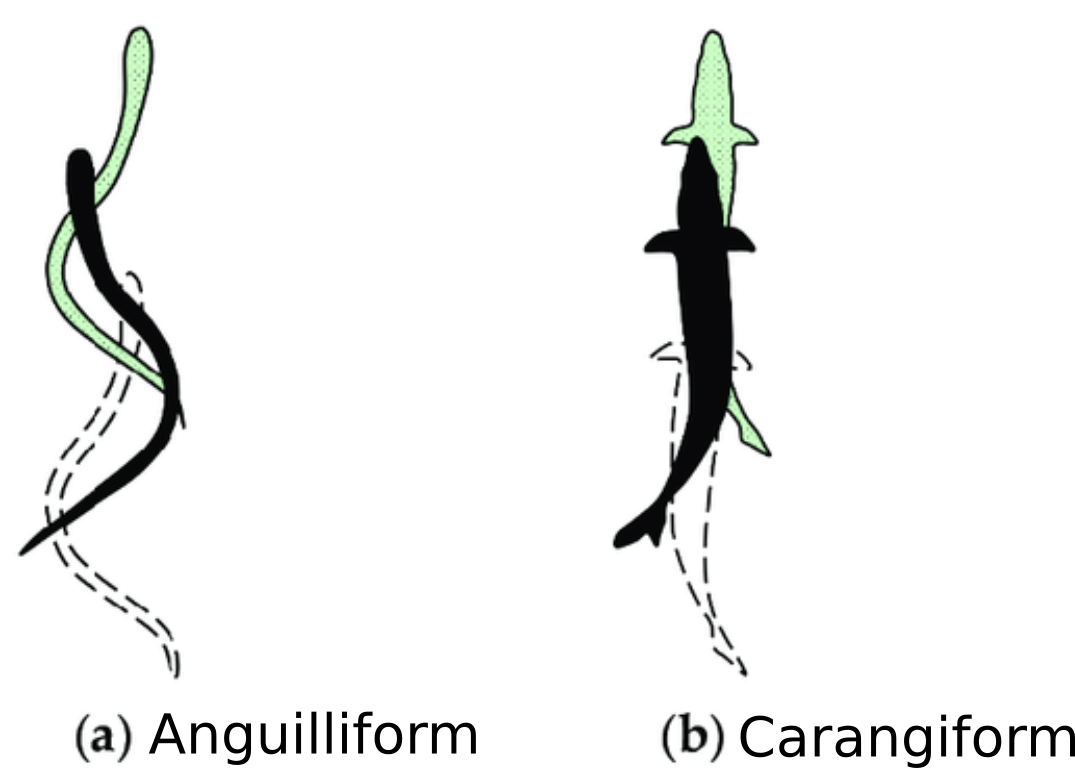
\includegraphics[width=0.5\textwidth]{figures/carangiform.png}
  \caption{\label{fig:carangiform} A snapshot of the body shape for an anguilliform (a) and carangiform (b) swimmer.}
\end{figure}

You will model the carangiform swimming mode of the zebrafish in this section with a double chain CPG oscillators and scaling the motor gains from the oscillators to the muscles. You will actively control the joints $i=0,...,12$, while the remaining left and right muscle activations ($M_{L_{13,14}}$ and $M_{R_{13,14}}$, i.e.; the tail joints) will be set to zero.

Here we first describe the equations of the abstract oscillator network you will implement to control the zebrafish. To model the spinal CPG controller, we consider two chains of $n_{cpg}=26$ populations of CPG neurons on each body side as shown in Fig \ref{fig:model_controller}, where each joint is governed by two oscillators.

\begin{figure}[H]
  \centering 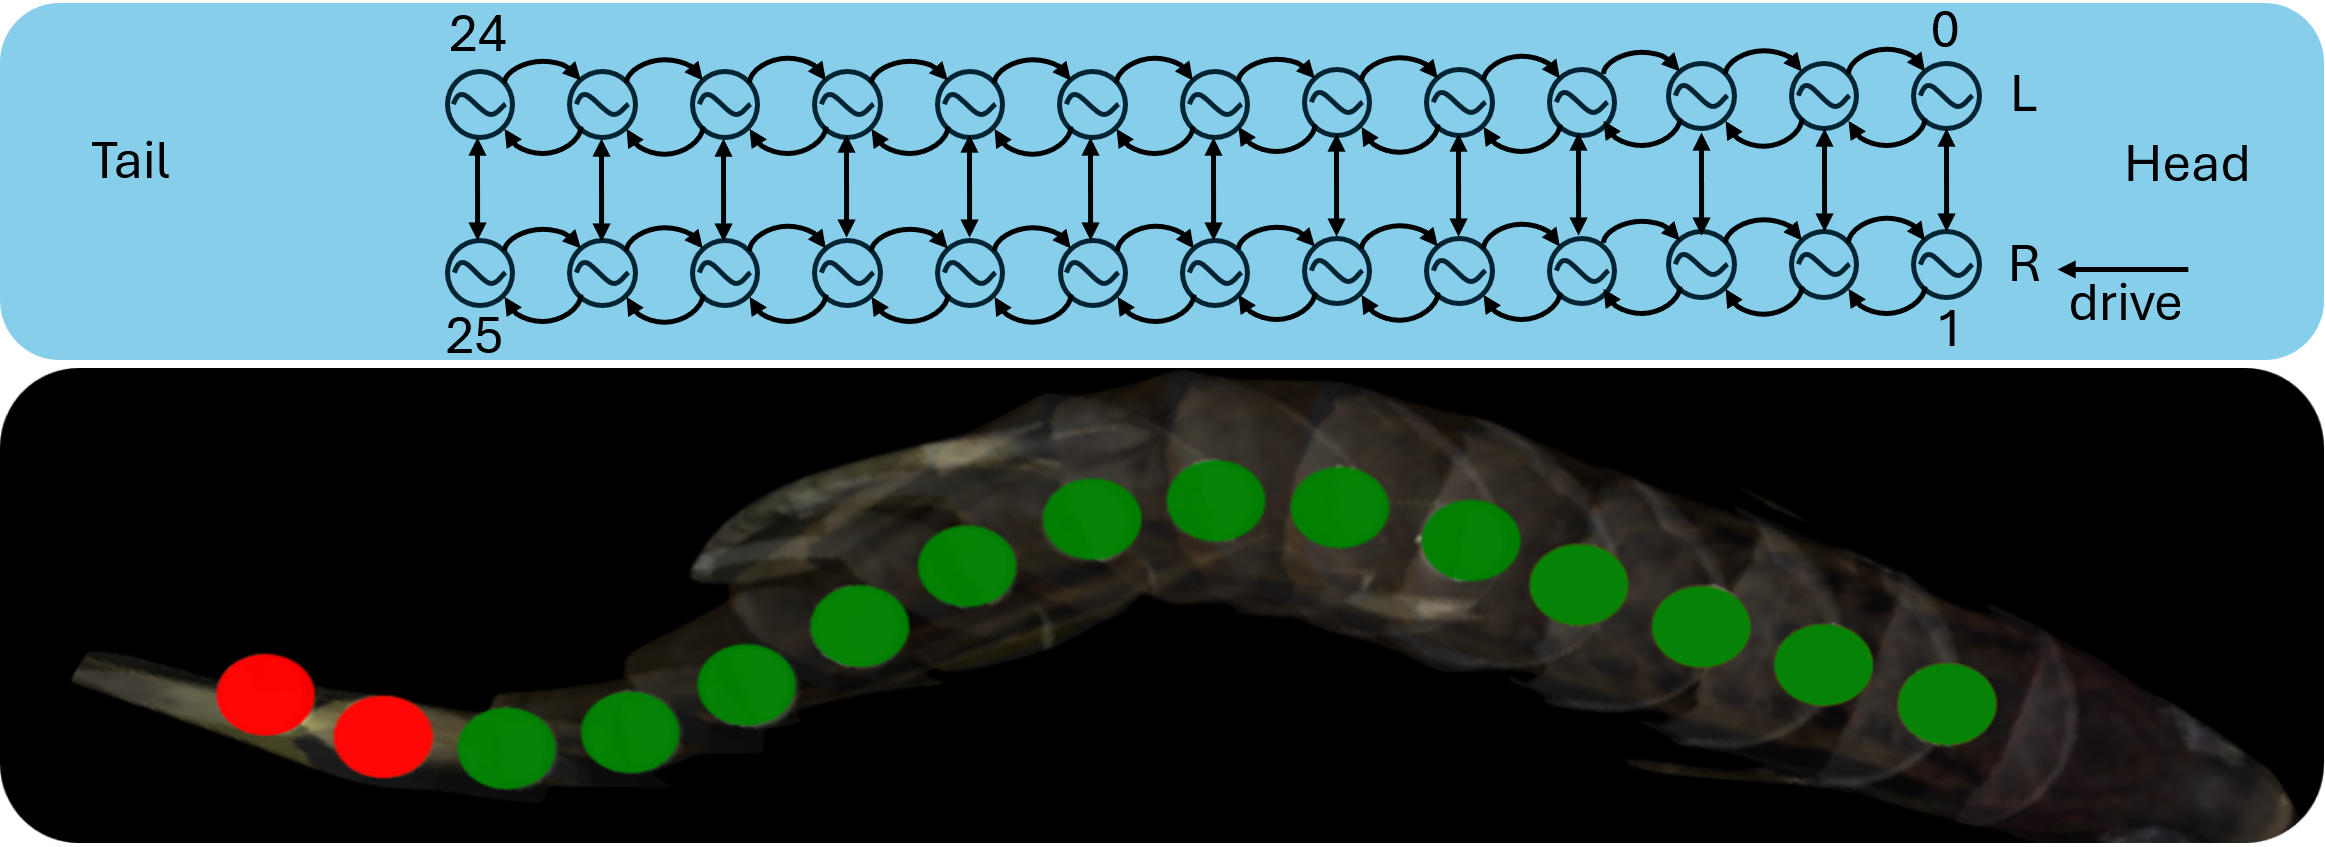
\includegraphics[width=.8\textwidth]{figures/model_controller.png}
  \caption{\label{fig:model_controller} Configuration of the spinal CPG controller in the zebrafish. The joints that you should actively control (joints 0-12) are marked in green and joints that should be left passive (joints 13-14) are marked in red. The active joints are driven by 13 pairs of Ekeberg muscles receiving motor outputs from a double chain of 26 oscillators with nearest-neighbor and contralateral coupling. The CPG model receives descending signals from the MLR region in the brain, which is represented as a drive signal in this model.}
\end{figure}

Let us index the left-side CPG units with the even index $i=0, 2,...,24$ and the right-side CPG units with the odd index $i=1, 3,...,25$. Each CPG unit is described by following equations:

The oscillator's phase equation is defined below, with $ \theta_i $ the oscillator phase, $f$ the frequency, $ w_{ij} $ the coupling
weights, $ \phi_{ij} $ the nominal phase lag (phase bias), $ r_i $ the
oscillator amplitude.
\begin{equation}
  \label{eq:dphase}
  \dot{\theta}_i = 2 \pi f + \sum_j r_j w_{ij} sin(\theta_j - \theta_i - \phi_{ij})
\end{equation}

In this model we only consider couplings between adjacent (i.e. successive segments) and contralateral (i.e. left-right) oscillators. The coupling weights are defined as below:

\begin{equation}
  \label{eq:dcw}
  w_{ij} =
    \begin{cases}
    w_{body2body},& \text{if } |i-j|=1 \text{ and } i,j \text{ on same side}\\
    w_{body2body\_contralateral}, & \text{if } |i-j|=n_{joint}
    \end{cases}
\end{equation}

The phase lags are defined as below, such that the phase lags between contralateral segments are constant $\pi$ and the phase lags between neighborhood segments are constant and sum up to $\phi_{body\_total}$ from head to tail. $n_{joints}$ here refer to the total number of body joints including the passive ones and assuming they would naturally follow the same phase lags as active joints. We connect $n$ oscillators with $n-1$ phase lags. Assuming a total phase lag of 1, we have to divide the total body phase lag by $n_{joint}-1$.

\begin{equation}
  \label{eq:phicw}
  \phi_{ij} =
    \begin{cases}
    sign(i-j)\cdot\frac{\phi_{body\_total}}{n_{joints}-1},& \text{if } |i-j|=1 \text{ and } i,j \text{ on same side}\\
    sign(i-j)\cdot\pi,& \text{if } |i-j|=n_{joint}
    \end{cases}
\end{equation}


The oscillator's amplitudes are defined below, with $ r_i $ the
oscillator amplitude, $ R_i $ the nominal amplitude and $ r_i $ the
convergence rate of nominal amplitudes. Note that this equation is actually the same equation as in \cite{ijspeert2007swimming} and has been simplified into a first-order ODE in order to simplify the implementation in this project.

\begin{equation}
  \label{eq:dr}
  \dot{r}_i = a (R_i - r_i)
\end{equation}

The oscillator frequency and nominal amplitudes are defined as linear functions of drive $d$ to simulate that the CPG controller can be receive descending commands from higher level controller (brain).

\begin{equation}
  \label{eq:amp}
  R_i = G_{amp\_i}\cdot d
\end{equation}
\begin{equation}
  \label{eq:freq}
  f = G_{freq}\cdot d + offset
\end{equation}

The motor output commands for the body joints are defined below, with $G$ a scaling factor for the motor output.
\begin{equation}
  \label{eq:output_body}
  q_i = G\cdot r_i(1 + cos(\theta_i))
\end{equation}


The meaning and default values of parameters mentioned above are given in Table \ref{table_par_CPG}.

\begin{table}[!ht]
\centering
\begin{tabular}{ l l l }
 Parameter & Meaning & Defaults \\
 $drive$ & Drive signal from the brain & 4\\
 $cpg\_frequency\_gain$ & Frequency gain of the oscillator (wrt. drive) & 0.6\\
 $cpg\_frequency\_offset$ & Offset of the oscillator frequency & 0.6\\
 $cpg\_amplitude\_gain$ & Nominal amplitude gain per oscillator (wrt. drive) & 0.125 (all)\\
 $weights\_body2body$ & Coupling weights between neighborhood oscillators & 30\\
 $weights\_body2body\_segment$ & Coupling weights between contralateral oscillators & 10\\
 $phase\_lag\_body$ & Total spine phase lag from head to tail& $2\pi$\\
 $amplitude\_rates$ & Convergence rate of nominal amplitudes& 1
\end{tabular}
\caption{Default values and biophysical meaning of the parameters of the abstract oscillator CPG equations}
\label{table_par_CPG}
\end{table}
\textbf{Questions:}

\textbf{\underline{Question 3.1} Implement the abstract oscillator model in \fileref{abstract\_oscillator\_controller.py}. Specifically, complete the function \fileref{network\_ode} , \fileref{motor\_output} and \fileref{step\_euler}.
    You can check \fileref{simulation\_parameters.py} which the controller file reads for parameter naming conventions and default values.}
\begin{itemize}
        \item \fileref{network\_ode}: In this function you have to implement Ordinary Differential Equation (ODE) to compute the evolution of oscillator phases and amplitudes. Specifically, refer to Eq.\ref{eq:dphase} , Eq.\ref{eq:dr} and relevant equations to compute the CPG parameters.
        \item \fileref{motor\_output}: In this function you use the network state at current iteration to compute the motor output as in Eq.\ref{eq:output_body} for the active joints. Then you store the computed motor output in \textit{motor\_out} for future analysis.
        \item \fileref{step\_euler}: In this function you perform an Euler integration time step of the oscillator states with the derivatives you computed in \fileref{network\_ode} (similar to what you have implemented in Lab 1). As a result you return the muscle activations for both the active joints (computed from updated network states in \fileref{motor\_output}) and passive joints.
    \end{itemize}

\textbf{\underline{Question 3.2} Test your implementation by running the network using \fileref{exercise\_3.py}. For the network parameters check lecture slides (pay attention to different number of segments). You can also	find more information in~\cite{ijspeert2007swimming} (especially in the supplementary material). You can set all the network parameters in the \fileref{simulation\_parameters.py} or override them by passing an argument to $all\_pars$. }

\textbf{\underline{Question 3.3} Report the controller and mechanical metrics of the simulation. Plot the oscillator phases evolution, oscillator amplitudes evolution, motor output and motor output difference evolution, and the zebrafish joint angles evolution vs time. Record a video of the zebrafish swimming for 5s with the abstract oscillator controller. You might need to change \textit{video\_record} and \textit{video\_name} to generate a video output.  }

\textbf{Hint:} Optionally you can use some helper functions such as \textit{plot\_time\_histories} to generate the plots. By default the code will try to use \href{https://ffmpeg.org/download.html}{ffmpeg} as the codec and you might have to install it and add it to PATH if not already.

\textbf{\underline{Question 3.4} Explore the effect of higher and lower drive parameter and report how the change of drive affects the abstract oscillator controller, the motor output, and the locomotion performance.  }



\subsection*{4. Optimization of swimming kinematics}

In the last section you worked on implementing an abstract oscillator to drive the zebrafish to generate some swimming behaviors. Yet the resulting kinematics can be far from the real animal kinematics if the controller parameters are not properly tuned. In this task we will optimize the nominal amplitude gains per joint (\textit{cpg\_amplitude\_gain}) to imitate the zebrafish kinematics in the real world (Fig \ref{fig:zebrafish_kinematics}).

\begin{figure}[H]
  \centering
    \hspace{-0.5cm}
    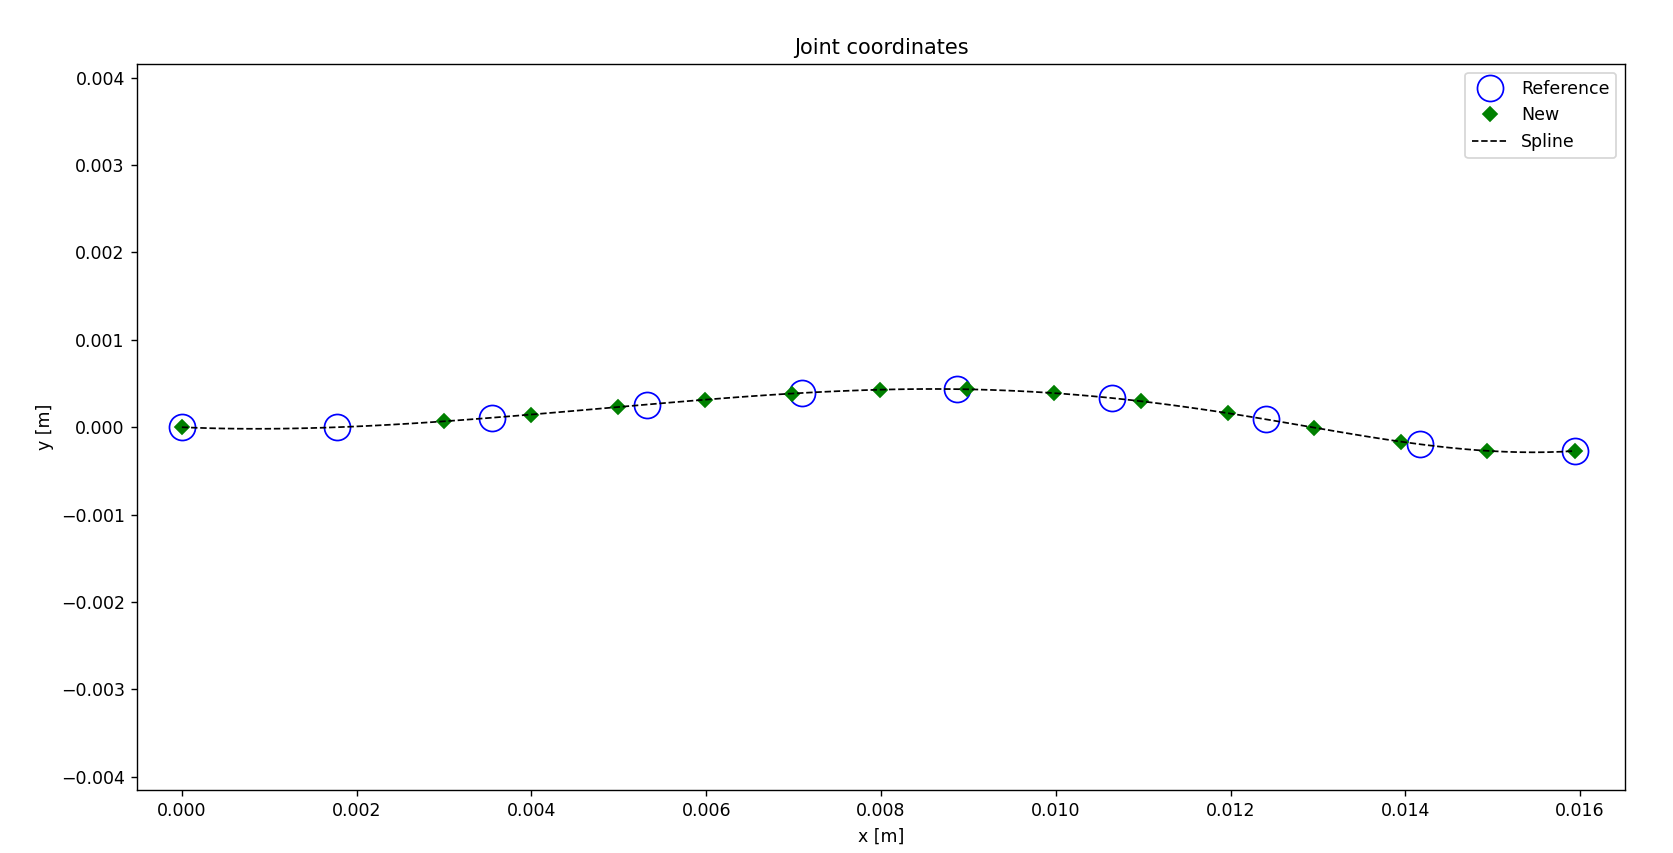
\includegraphics[width=.5\textwidth]{figures/joint_fitting.png}
    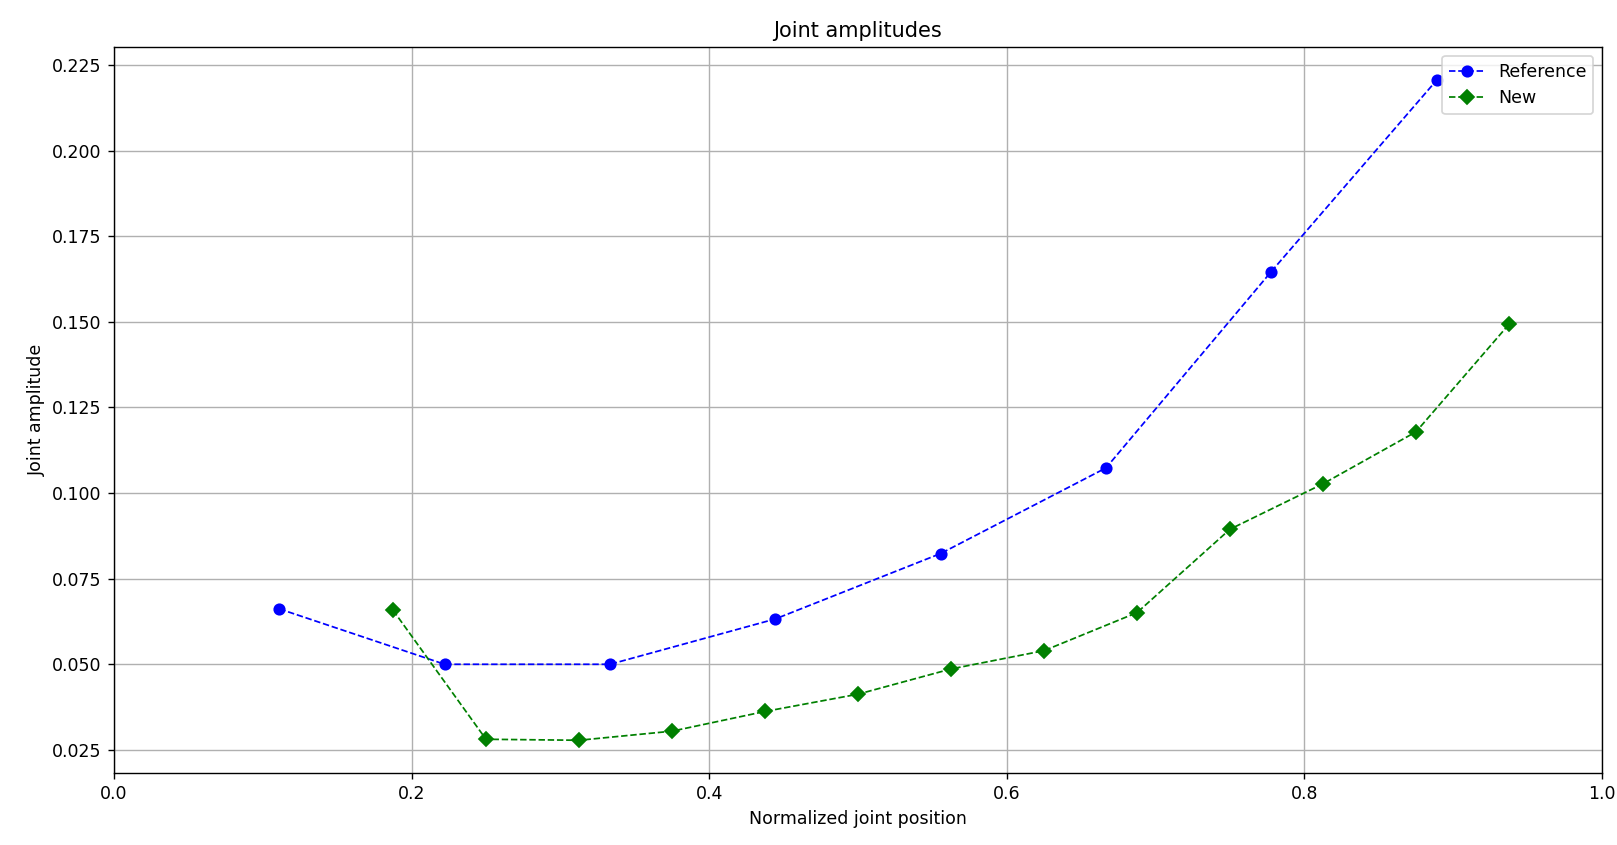
\includegraphics[width=.5\textwidth]{figures/joint_kinematics_observed_fitted.png}

  \caption{
  \label{fig:zebrafish_kinematics} \textbf{Left:} Tracked kinematics of zebrafish (blue circle) and interpolated kinematics of the model (green dots). \textbf{Right:} Tracked joint angles of zebrafish (blue circle) and interpolated joint angles according of the model (green dots) in \textbf{radians}
  }

\end{figure}

From Eq.~\ref{eq:phicw}, we apply a phase lag of $\pi$ between contralateral body segments so the left and right muscle activations are anti-phase. Therefore, the resulting joint torque as the difference between the left and right muscle torque is correlated with the amplitudes of the motor output as well as the oscillator amplitudes. We could update the nominal amplitude gains per joint based on the difference between the desired joint amplitudes and the obtained joint amplitudes from simulation results.

Here we provide the 3 pseudo-steps for the optimization algorithm you have to implement. The details of each step are explained below:

\begin{algorithm}[H]
\caption{Gradient Descend}\label{euclid}
\begin{algorithmic}[1]
\While {$ error_{joint\_amp}> tolerance$ \textbf{and} $iter$ < $iter_{max}$}
\State Update the nominal amplitude gain
\State Simulate and store the simulation result
\State Compute current joint amplitude errors
\EndWhile
\end{algorithmic}
\end{algorithm}


\textbf{Update the nominal amplitude gain: }Here we update the nominal amplitude gain with a scaling method. The method scales the old nominal amplitude gain based on the proportion between the actual and reference joint amplitudes. If the actual joint amplitudes are greater than the reference ones, the motor gain will be scaled with a factor within $[0,1]$. Otherwise, the motor gain will be scaled up with a factor within $[1,\infty]$. Note that the learning rate  should be a positive value within $lr\in[0,1]$ to avoid flipping the sign of the motor gain.
\begin{equation}
  \label{eq:mo_gain_update}
  motor_{gain\_new} = motor_{gain\_old} * (1 + lr*(-1+\frac{A_{ref}}{A_{res}}))
\end{equation}
\textbf{Simulate and store the simulation result:} Here you initialize \fileref{Simulation parameters} with the updated nominal amplitude gains (pass this as an argument to overide the default parameters) and run the simulation with \fileref{run\_single}.

\textbf{Hint:} To organize the simulation result from different trials, You can pass $simulation\_i$ as an additional argument to \fileref{Simulation parameters}, which will index the simulation trials in the logged outputs with a suffix.

\textbf{Compute current joint amplitude errors:} Here you read back the simulation result you saved in last step. They are located under $log\_path$ of the \fileref{Simulation parameters}. Load the controller with \fileref{load\_object} function and use the joint amplitude metrics. Compare the result with the reference joint amplitudes stored in \fileref{REF\_JOINT\_AMP} and compute the current joint error $error\_{joint\_amp}$.

\textbf{\underline{Question 4.1} Implement the optimization algorithm in \fileref{exercise\_4.py}. }

\textbf{\underline{Question 4.2} Optimize the nominal amplitude gain so that the difference between the simulation result and the reference is less than 1\%. Plot the joint angles of the optimized controller vs time. Plot an overlay of reference joint amplitudes. }

\textbf{\underline{Question 4.3} Report the controller and mechanical metrics of the optimized controller. Record a video of the zebrafish swimming for 5s. What do you observe with the optimized controller compared to the unoptimized one and how does the metrics change? }

% \subsection*{5. Open question}\label{sec:ex9}
% Open questions. These questions are meant to assess your understanding of the topics addressed during the project. You should reply in a concise, scientific way by explaining your reasoning and listing the reference literature to support your idea.

% \begin{enumerate}
% \item During the project, you tested the effect of proprioceptive sensory feedback with varying levels of noise. How would you design a biological experiment to validate in-vivo the simulation results?
% \item What other aspects of zebrafish locomotion could be affected by the presence (or absence) of proprioceptive sensory feedback? How would you test those hypotheses in simulation and biological experiments?
% \item What other types of sensory feedback could play a role during zebrafish locomotion? How would you disambiguate the relative contribution of the different sensory feedback modalities? How can simulation help in addressing this problem?
% \end{enumerate}



%% -----------------------------SOLUTION ------------------------------


\bibliographystyle{ieeetr}
\bibliography{project1}
\label{sec:references}





% \newpage

% \section*{APPENDIX}
% \label{sec:appendix}

\end{document}

%%% Local Variables:
%%% mode: latex
%%% TeX-master: t
%%% End: